%----------------------------------------------------------------------------------------
%	PACKAGES AND OTHER DOCUMENT CONFIGURATIONS
%----------------------------------------------------------------------------------------
\documentclass[11pt, a4paper]{article}

%\usepackage[french]{babel}
%\usepackage{mathpazo} % Use the Palatino font
%\usepackage{booktabs} % Required for better horizontal rules in tables
\usepackage{float} % Required for including images
\usepackage{geometry} %Required for changing the size of the marge
\usepackage[utf8]{inputenc} % Required for inputting international characters
\usepackage[T1]{fontenc} % Output font encoding for international characters
\usepackage{graphicx} % Required for including images
\usepackage{listings} % Required for insertion of code
\usepackage{enumerate} % To modify the enumerate environment
\usepackage{xcolor} % Required to add color in text
\usepackage{titling} % Easy access to assignement information

%----------------------------------------------------------------------------------------
%	DEFINE SYNTAX COLOR TO OUTPUT CODE
%----------------------------------------------------------------------------------------

\definecolor{codegreen}{rgb}{0,0.6,0}
\definecolor{codegray}{rgb}{0.5,0.5,0.5}
\definecolor{codepurple}{rgb}{0.58,0,0.82}
\definecolor{backcolour}{rgb}{0.95,0.95,0.95}

\lstdefinestyle{mystyle}{
backgroundcolor=\color{backcolour},   
commentstyle=\color{codegreen},
keywordstyle=\color{magenta},
numberstyle=\tiny\color{codegray},
stringstyle=\color{codepurple},
basicstyle=\ttfamily\footnotesize,
breakatwhitespace=false,         
breaklines=true,                 
captionpos=b,                    
keepspaces=true,                 
numbers=left,                    
numbersep=5pt,                  
showspaces=false,                
showstringspaces=false,
showtabs=false,                  
tabsize=2
}

\lstset{style=mystyle}

%----------------------------------------------------------------------------------------
%	ASSIGNMENT INFORMATION
%----------------------------------------------------------------------------------------
\author{RACINE Florian}
\title{Prise de note lecture informatique}
\setcounter{tocdepth}{5} % Profondeur pour le sommaire
\geometry{hmargin=2.5cm,vmargin=1.5cm}

%----------------------------------------------------------------------------------------
%	DEFINE COMMANDS
%----------------------------------------------------------------------------------------
\newcommand{\HRule}{\rule{\linewidth}{0.5mm}}

\begin{document}
%----------------------------------------------------------------------------------------
%	COVER PAGE
%----------------------------------------------------------------------------------------
\maketitle % Output the assignment title, created automatically using the information in the custom commands above
\vspace*{\stretch{1}}
\begin{center}
\HRule \\[0.4cm]
{ \huge \bfseries \thetitle \\[0.4cm] }
\HRule \\[2cm]
\graphicspath{{/home/evo/Pictures/logo/}}
\includegraphics[width = 7cm]{logo}
\end{center}
\vspace*{\stretch{1}}
\newpage

%----------------------------------------------------------------------------------------
%	TABLE OF CONTENTS
%----------------------------------------------------------------------------------------
\tableofcontents
\newpage

\graphicspath{{image/}} % Changing the path to include image

%----------------------------------------------------------------------------------------
%	SECTION 1
%----------------------------------------------------------------------------------------
\section{Algorithmie}
\subsection{Introduction à l'algorithmique}
\subsubsection{Introduction}
Cet ouvrage sans équivalent, exhaustif et d'accès facile est une introduction complète à l'algorithmique et s'adresse aussi bien aux étudiants qu'aux progessionnels en informatique.
\newline
L'éventail des algorithmes étudiés dans ce livre va des plus classiques, commes les algoritmes de tri et les fonctions de hachage, aux plus récents comme ceux de l'algorithmique parallèle, permettant ainsi de passer progressivement des notions élémentaires aux thèmes les plus pointus.

\subsubsection{Tri rapide}
\paragraph{Introduction}
 Cet algorithme appelé ALGORITHME TRI RAPIDE(QuickSort)
 il s'agit d'ordonner le tableau à partir d'un pivot (valeur
 choisie dans le tableau (généralement la première valeur)
 Dans ce mêmetableau on classe à gauche les valeurs inférieurs et
 à droite les valeurs supérieurs.
 Ensuite on rappelle l'ALGORIHTME TRI RAPIDE,
 une fois pour la partie gauche, une fois pour la partie droite.
 Là est la récursivité.
 \paragraph{Complexité}
 En moyenne la complexité est de nlog(n) ce qui en fait si on ne connait aucune information sur la liste à trier le meilleur tri.
 Dans le pire des cas la complexité est de $n^{2}$ mais cela est très peu probable d'autant plus si le pivot est choisi aléatoirement.
 \begin{figure}[h]
     \centering
     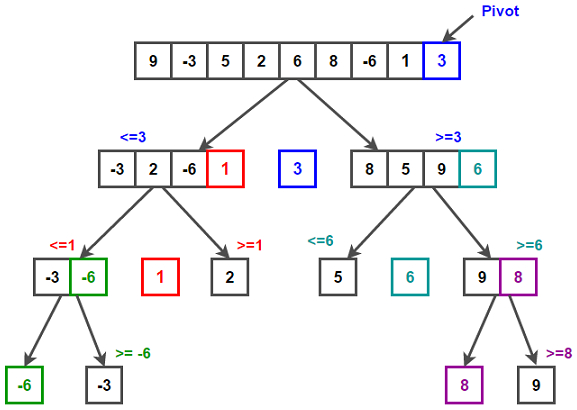
\includegraphics[width=0.8\textwidth]{shemaTriRapide}
     \caption{shemaTriRapide}
     \label{fig:shemaTriRapide}
 \end{figure}
 \newpage
 \paragraph{Exemple}
 Proposition d'implémentation d'ALGORITHME TRI RAPIDE:
\begin{lstlisting}[language=C]
#include <stdio.h>
#include <stdlib.h>
#include <time.h>
/* Programme principal
 */
int main()
{
 int taille_1=10;
 int tableau[taille_1];
 int i;
 /* Saisie par l'operateur des valeurs entieres dans le tableau */
 init_tab(tableau,0,taille_1);
 /* Tri du tableau */
 tri_tab_recursif(tableau,0,taille_1);
 /* Affichage du tableau trie */
 for(i=0;i<taille_1;i++) {printf("%d ",tableau[i]);}
 putchar('\n');
}
/* fonction qui permet à l'operateur de saisir sa liste de nombres
 */
void init_tab(int tab[], int deb, int taille)
{
 int i;
 for(i=deb; i < taille; i++)
 {
 printf("valeur %d : ",i);
 scanf("%d", &tab[i]);
 }
}
/* fonction de tri RECURSIF
 */
void tri_tab_recursif(int tab[],int deb,int fin)
{
 const int pivot = tab[deb];
 int pos=deb;
 int i;
 if (deb>=fin)
 return;
/* cette boucle permet de placer le pivot (debut du tableau à trier)
 au bon endroit dans le tableau
 avec toutes les valeurs plus petites avant
 et les valeurs plus grandes apres
 à la fin, la valeur pivot se trouve dans le tableau à tab[pos]
 */
 for (i=deb; i<fin ; i++)
 {
 if (tab[i]<pivot)
 {
 tab[pos]=tab[i];
 pos++;
 tab[i]=tab[pos];
 tab[pos]=pivot;
 }
 }
/* Il ne reste plus qu'a rappeler la procedure de tri
 sur le debut du tableau jusquà pos (exclu) : tab[pos-1]
 */
 tri_tab_recursif(tab,deb,pos);
/* et de rappeler la procedure de tri
 sur la fin du tableau à partir de la premiere valeur apres le pivot
 tab[pos+1]
 */
 tri_tab_recursif(tab,pos+1,fin);
}
\end{lstlisting}
\newpage
\subsubsection{Tri linéaire}
\paragraph{Introduction}
Dans un tri comparatif, on se sert uniquement de comparaisons entre les éléments pour obtenir des informations sur l'ordre d'une séquence d'entrée.
Ces type de tris sont contraint à une complexité d'au moin n*log(n).
Les tris linéaires sont des tris faisant appel à d'autre opération que les comparaisons.
Par exemple, le tri par base, le tri par paquets, le tri par dénombrement\ldots
\paragraph{Tri par denombrement (ou tri comptage)}
Ce tri troc de la complexité contre de l'espace mémoire. Complexité moyenne : O(n)
\newline
Le tri par dénombrement suppose que chacun des n éléments d'entrée est un entier de l'intervalle 1 à k, pour un entier k donné. Lorsque k = O(n), le trie s'exécute en O(n).
\newline
Le principe du tri par dénombrement est de déterminer pour chaque élément de l'entrée, le nombre d'élément inférieurs à x. Cette information peut servie à placer l'élément x directement à sa position dans le tableau de sortie. Par exemple, s'il existe 17 éléments inférieurs à x, alors x se trouvera en sortie à la position 18.
\begin{lstlisting}[language=C++]
public class CountingSort
{
    public static void SortCounting(int[] input, int min, int max)
    {
        var count = new int[max - min + 1];
        var z = 0;

        for (var i = 0; i < count.Length; i++)
            count[i] = 0;

        foreach (int i in input)
            count[i - min]++;

        for (var i = min; i <= max; i++)
        {
            while (count[i - min]-- > 0)
            {
                input[z] = i;
                ++z;
            }
        }
    }

    public static int[] Main(int[] input)
    {
        SortCounting(input, input.Min(), input.Max());
        return input;
    }
}
\end{lstlisting}
\begin{figure}[h]
    \centering
    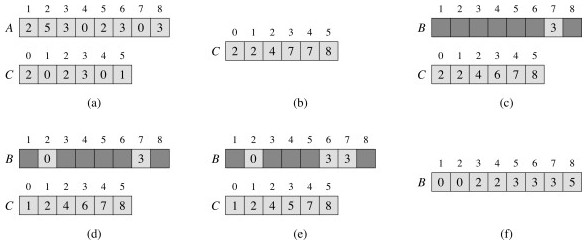
\includegraphics[width=0.8\textwidth]{graphTriComptage}
    \caption{graphTriComptage}
    \label{fig:graphTriComptage}
\end{figure}
\paragraph{Tri Base}
Le principe du Tri base est de classer successivement les nombres à trier par chiffre les moins significatifs (pas très intuitif).
Il repose donc sur un autre algorithme de trie pour trier les nombres par chiffre.
\begin{figure}[h]
    \centering
    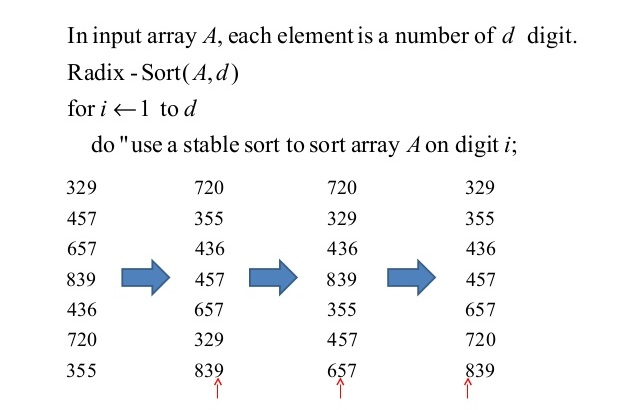
\includegraphics[width=0.8\textwidth]{graphTriBase}
    \caption{graphTriBase}
    \label{fig:graphTriBase}
\end{figure}    
\end{document}
